%S_parameter
Normally an electrical network can be considered as a 'black box', which contains amounts of interconnected basic electrical circuit components such as resistors, capacitors, inductors and transistors etc. On this 'black box' may exist many ports, which connect with other circuits. In order to describe the characteristics of this network H-Parameters are used, which describe the relation between voltages and currents of each two ports. In Fig. \ref{fig:2_port_network} is a 2-port network $V_{1}$ and $V_{2}$ are total voltages of both ports; $I_{1}$ and $I_{2}$ are total currents of both ports respectively.\\
 
\begin{figure}[!ht]
\centering
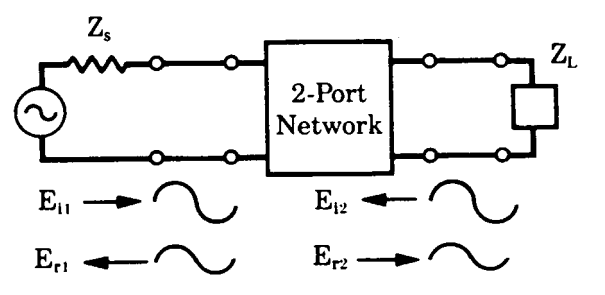
\includegraphics[width=0.6\textwidth]{bilder/s_parameters}
\caption{2-Port-Network \cite{aglient_s_parameters}.}
\label{fig:2_port_network}
\end{figure}
Relations between voltages and currents are given by %(\ref{eq:voltage_current1}-\ref{eq:voltage_current2}). 
\begin{equation}
V_{1}=h_{11}I_{1}+h_{12}V_{2} \text{,}
\label{eq:voltage_current1}
\end{equation}
\begin{equation}
I_{2}=h_{21}I_{1}+h_{22}V_{2} \text{.}
\label{eq:voltage_current2}
\end{equation}
Where $h_{11},h_{12},h_{21}$ and $h_{22}$ are H-Parameters and defined as %(\ref{eq:h_parameters1}-\ref{eq:h_parameters2}).
\begin{align*}
h_{11}&=\frac{V_{1}}{I_{1}}|_{V_{2}=0}\quad\text{,} h_{12}=\frac{V_{1}}{V_{2}}|_{I_{1}=0}\text{,}
%\label{eq:h_parameters1}
\\
h_{21}&=\frac{I_{2}}{I_{1}}|_{V_{2}=0}\quad\text{,} h_{22}=\frac{I_{2}}{V_{2}}|_{I_{1}=0}\text{.}
%\label{eq:h_parameters2}
\end{align*}
But H-Parameters cannot always be calculated for microwave circuits. Agilent\cite{aglient_s_parameters} has listed some problems of H-Parameters in high frequency:
\begin{itemize}
\item It is not easy to measure the total voltage and total current at the ports of the network.
\item Short and open circuits are not always available for a broad frequency band.
\item For high frequency some circuit are not stable in short or open conditions.
\end{itemize}
Scattering parameters or S-parameters are perfect description of microwave circuit\cite{RF194_s_parameters}. In that case traveling waves are applied instead of total voltages and currents. $E_{i1}$ and $E_{i2}$ represent incidence waves over left and right ports of the network respectively. $E_{r1}$ and $E_{r2}$ are reflective waves. The relation between traveling waves, total voltages and currents has relations %(\ref{eq:voltage_wave1}-\ref{eq:voltage_wave2}).
\begin{align}
V_{1}&=E_{i1}+E_{r1}\text{,}\quad V_{2}=E_{i2}+E_{r2}\text{,}
\label{eq:voltage_wave1}\\
I_{1}&=\frac{E_{i1}-E_{r1}}{Z_{0}}\text{,}\quad I_{2}=\frac{E_{i2}-E_{r2}}{Z_{0}}\text{.}
\label{eq:voltage_wave2}
\end{align}
Traveling waves themselves can be expressed in terms of H-Parameters (\ref{eq:er1}-\ref{eq:er2}). 
\begin{align}
E_{r1}&=f_{11}(h)E_{i1}+f_{12}(h)E_{i2}
\label{eq:er1}
\\
E_{r2}&=f_{21}(h)E_{i1}+f_{22}(h)E_{i2}
\label{eq:er2}
\end{align}
Here $f11, f12, f21, f22$ are the network parameters, which indicate the relation between traveling voltages waves and total voltages or currents. If both sides of the functions (\ref{eq:er1}-\ref{eq:er2}) are divided by $\sqrt{Z_{0}}$ ($Z_{0}$ system impedance) a new set of variables can be obtained
\begin{align} 
a_{1}&=\frac{Ei1}{\sqrt{Z_{0}}}=\frac{V_{1}+I_{1}Z_{0}}{2\sqrt{Z_{0}}} \text{,}\quad a_{2}=\frac{Ei2}{\sqrt{Z_{0}}}=\frac{V_{2}+I_{2}Z_{0}}{2\sqrt{Z_{0}}} \\
b_{1}&=\frac{Er1}{\sqrt{Z_{0}}}=\frac{V_{1}-I_{1}Z_{0}}{2\sqrt{Z_{0}}}  \text{,}\quad b_{2}=\frac{Er2}{\sqrt{Z_{0}}}=\frac{V_{2}-I_{2}Z_{0}}{2\sqrt{Z_{0}}}
\end{align}
So relations of the new variables are given by:
\begin{align}
b_{1}&=S_{11}a_{1}+S_{12}a_{2}\\
b_{2}&=S_{21}a_{1}+S_{22}a_{2}
\end{align}
or in matrics form:
\begin{equation}
		\begin{pmatrix}
			b_{1}&\\
			b_{2}&
		\end{pmatrix}
	=	
		\begin{pmatrix}
			S_{11}&S_{12}\\
			S_{21}&S_{22}
		\end{pmatrix}
		\begin{pmatrix}
			a_{1}&\\
			a_{2}&
		\end{pmatrix}
\label{eq:s_matrix}
\end{equation}

The S-Parameters are defined as following:
\begin{align*}
S_{11}&=\frac{b_{1}}{a_{1}}|_{a_{2}=0}\\
S_{21}&=\frac{b_{2}}{a_{1}}|_{a_{2}=0}\\
S_{22}&=\frac{b_{2}}{a_{2}}|_{a_{1}=0}\\
S_{12}&=\frac{b_{1}}{a_{2}}|_{a_{1}=0}
\end{align*}
The phical meaning of the S-Parameters are described as following:
\begin{itemize}
\item $S_{11}$ is the input port reflection coefficient
\item $S_{12}$ is the reverse transmission coefficient
\item $S_{21}$ is the forward transmission coefficient
\item $S_{22}$ is the output port reflection coefficient
\end{itemize}
Here $|S_{21}|$ is often used to estimate the transmission ability of a network. Therefore $|S_{21}|$ equals the coupling efficiency in this work.
